\documentclass[twocolumn,english]{IEEEtran}
\usepackage[T1]{fontenc}
\usepackage{babel}
\usepackage{amsthm}
\usepackage{amsmath}
\usepackage{graphicx}
\usepackage[unicode=true,
 bookmarks=true,bookmarksnumbered=true,bookmarksopen=true,bookmarksopenlevel=1,
 breaklinks=false,pdfborder={0 0 0},backref=false,colorlinks=false]
 {hyperref}
\usepackage{bm}
\usepackage{amsmath}
\usepackage{amssymb}
\usepackage{natbib}
\usepackage{array}
\usepackage{calc}
\newcolumntype{W}{>{\centering\arraybackslash}m{25mm}}
\newcolumntype{L}{>{\centering\arraybackslash}m{15mm}}


\hypersetup{
 pdftitle=  {Lab 3: Digital Oscilloscope Memo},
 pdfauthor= {Zack Garza, Shawn Azam, Nick Lonsdale},
 pdfpagelayout=OneColumn, pdfnewwindow=true, pdfstartview=XYZ, plainpages=false}

\makeatletter


%%%%%%%%%%%%%%%%%%%%%%%%%%%%%% Textclass specific LaTeX commands.
 % protect \markboth against an old bug reintroduced in babel >= 3.8g
 \let\oldforeign@language\foreign@language
 \DeclareRobustCommand{\foreign@language}[1]{%
   \lowercase{\oldforeign@language{#1}}}
\theoremstyle{plain}
\newtheorem{thm}{\protect\theoremname}
\theoremstyle{plain}
\newtheorem{lem}[thm]{\protect\lemmaname}

%%%%%%%%%%%%%%%%%%%%%%%%%%%%%% User specified LaTeX commands.
% for subfigures/subtables
\ifCLASSOPTIONcompsoc
\usepackage[caption=false,font=normalsize,labelfont=sf,textfont=sf]{subfig}
\else
\usepackage[caption=false,font=footnotesize]{subfig}
\fi

\makeatother
\providecommand{\lemmaname}{Lemma}
\providecommand{\theoremname}{Theorem}
\setcounter{topnumber}{2}
\setcounter{bottomnumber}{2}
\setcounter{totalnumber}{4}
\renewcommand{\topfraction}{0.85}
\renewcommand{\bottomfraction}{0.85}
\renewcommand{\textfraction}{0.15}
\renewcommand{\floatpagefraction}{0.7}
\usepackage{float}
\begin{document}

\title{Digital Oscilloscope Memo}


\author{Shawn Azam, Nick Lonsdale, Zack Garza}


\IEEEspecialpapernotice
{Engineering 17L\\
Effective Date of Report: March 18, 2014}


\markboth{Digital Oscilloscope Memo}{Zack Garza, Shawn Azam, Nick Lonsdale}
\maketitle
\begin{abstract}
\IEEEPARstart{T}{he} purpose of this memo is to discuss several parameters on the digital oscilloscope and how they effect readings and measurements. The oscilloscope will then be used to simultaneously measure two channels of information from an LRC circuit to observe the circuit's response to a range of frequencies.
\end{abstract}

\tableofcontents

\section{Methodology}
\begin{enumerate}
 \item The signal generator was initialized with the frequency given in Table~\ref{tb:given_parameters} and connected to channel 1 of the oscilloscope.
 \item The self-calibration function on the oscilloscope was activated. The probes were then calibrated as well.
 \item The circuit shown in~\ref{fig:circuit} was constructed, with the initial values described in Table~\ref{tb:given_parameters}. Several settings were modified, and the changes and effects were recorded.
 \item Using the auto-measuring display, the values in Table~\ref{tb:parameter_error} were recorded.
\end{enumerate}

\begin{figure}[h!]
  \begin{centering}
  \begin{center}
  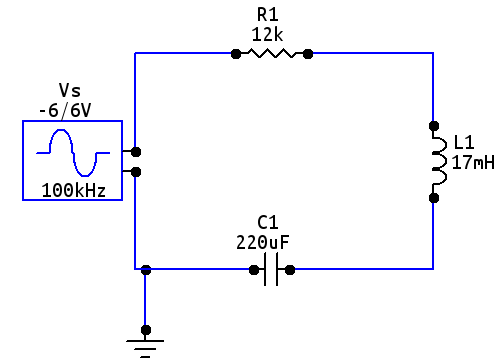
\includegraphics[width=\linewidth]{./Images/given_circuit.png}
  \label{fig:circuit}
  \caption{Theoretical circuit model.}
  \end{center}
  \par\end{centering}
  \end{figure}

\begin{table}[h!]
\centering{}
\caption{Lab Parameters (Given)}
\label{tb:given_parameters}
\begin{tabular}{|c|c|}
\hline
\textbf{Wave Type}                                                       & Sine      	\\ \hline
\textbf{Frequency}                                                       & 100 kHz   	\\ \hline
\textbf{\begin{tabular}[c]{@{}c@{}}Peak to Peak \\ Voltage\end{tabular}} & 12 V      	\\ \hline
\textbf{Resistance}                                             & 12k$\Omega$ 	\\ \hline
\textbf{Inductance}                                             & 17 mH     	\\ \hline
\textbf{Capacitance}                                            & 220$\mu$F  	\\ \hline
\textbf{DC Offset}							 & 0 V		\\ \hline
\end{tabular}
\end{table}

\begin{table}[h!]
\centering{}
\caption{Measured Values}
\label{tb:parameter_error}
\begin{tabular}{|c|c|c|}
\hline
\textbf{Parameter}	&\textbf{Measured Value}	&\textbf{Percent Error}	\\ \hline
Frequency		& (100 $\pm 0.2$) kHz		&0.2\%		\\ \hline
{Resistance}		& 12.12 k$\Omega$  		&1.0\% 		\\ \hline
{Inductance}		& 17.1 $\mu$H   		&0.6\% 		\\ \hline
{Capacitance}		& 222 $\mu$F  			&0.9\%		\\ \hline
\end{tabular}
\end{table}

\section{Data and Analysis}
\subsection{Oscilloscope Parameter Variations}
The following settings on the oscilloscope were adjusted, and the observed effects are explained below.

\noindent\textbf{AC / DC Coupling: }

Changing the coupling mode for this circuit did not exhibit a large change in the oscilloscope reading. This is largely due to the fact that the AC power source used did not have a DC offset. In DC coupling mode, the waveform will tend to oscillate about some positive voltage, i.e, the DC offset. By using AC coupling, the DC portion of the signal is blocked, and the waveform is shown oscillating about 0 volts instead. This can be useful for measuring small perturbations in AC measurements, as it serves as a noise gate that filters the signal and allows for more precise measurements at high magnifications.

\noindent\textbf{1x / 10x Probe: }

The probe is a device that allows the user to connect straight to the actual circuit, much like a multimeter, and measure the voltage across an element on the same screen as the oscilloscope. The probe used in this lab had a switch located on the handle that went from 1x to 10x. This switch makes the probes impedance on the circuit greater by 10 which in return decreases the voltage that the oscilloscope picks up by 10.

This capability is extremely useful when trying to minimize the amount of error caused by the probes resistance, especially if it is on the same order of magnitude as the resistances used in the circuit. There are many probes out there that have ranges greater than this one and those can be used in specific cases to lessen the errors caused by the probe.

\noindent\textbf{Invert On / Off}

On the oscilloscope there is a setting that allows the user to invert the wave about the x-axis. This would effectively reverse the sign of the voltages on a given channel, meaning positive voltages are negative and vice-versa. This setting can be used for comparing certain signals to see if they are exactly $180^{\circ}$ out of phase. If invert was used on this instance then the waves would line up exactly.

\subsection{Auto Measuring}
\begin{align*}
 &\text{RMS Voltage: \underline{$4.17$ V}}	&\text{Peak to Peak Amplitude: \underline{$11.8$ V}} 	\\
 &\text{Period: \underline{$1$ ms}} 		&\text{Frequency: \underline{$(100 \pm 0.2)$ kHz}}	\\
\end{align*}

\subsection{Triggering}
\begin{align*}
 \text{Triggering Type:}&	&\text{\underline{Edge}}\\
 \text{Triggering Source:}&	&\text{\underline{Ch. 2}}\\
 \text{Triggering Mode:}&	&\text{\underline{Auto}}
\end{align*}

The trigger level dictates at what point the oscilloscope begins measuring a signal. It can be set so that measurement does not begin until some condition is met, such as the presence of a specific level of voltage. This allows for finer control of capturing data. In Edge mode, the trigger is set to activate at the edge of a signal -- in this case, when the sine wave rises or falls. The trigger can be set to activate when the voltage condition is met and is either increasing or decreasing. The voltage level at which this occurs can be set via a knob on the scope, and the signal source can be set via the menu system.

It is possible for a circuit to never meet the initial trigger conditions -- in this case, the AUTO triggering setting forces the oscilloscope to automatically trigger after a certain amount of time, even if the input conditions are not met. This ensures that a minimum amount of measurements per second will be taken.

\subsection{Signals From Two Channels}
The component from the circuit chosen for measurement on Channel 2 was the $17$ mH capacitor. The frequency was lowered in order to exhibit a discernible response in the capacitor, and the following measurements were taken with a $35.2$ Hz sine wave. \\


\noindent Peak to Peak measurements for both channels:
\begin{align*}
 &\text{Ch.1 Peak to Peak (Source): }		&\text{\underline{$12.0$ V}}	\\
 &\text{Ch.2 Peak to Peak (Capacitor): }	&\text{\underline{$23.4$ mV}}	\\
 &\text{Period}		&\text{\underline{28.44 ms}}
\end{align*}

\begin{figure}[h!]
  \begin{centering}
  \begin{center}
  \includegraphics[width=\linewidth]{./Images/cam.png}
  \label{fig:source_voltage}
  \caption{Display of source waveform on the oscilloscope.}
  \end{center}
  \par\end{centering}
  \end{figure}

\noindent Phase shift between both channels:
\begin{align*}
 &\Delta t = 7.000\text{ms}	&\theta \approx 1.546\text{ rad} = 88.58^{\circ}
\end{align*}
Where $\theta$ is given by  $2\pi\frac{\Delta t}{T}$ or $2\pi f \Delta t$ in radians ($360\frac{\Delta t}{T}$ in degrees), $\Delta t$ is the distance in the time domain between two identical points on the adjacent waves, $T$ is the period (time in seconds between identical points on a waveform), and $f$ is the frequency of the generator.

\begin{figure}[h!]
  \begin{centering}
  \begin{center}
  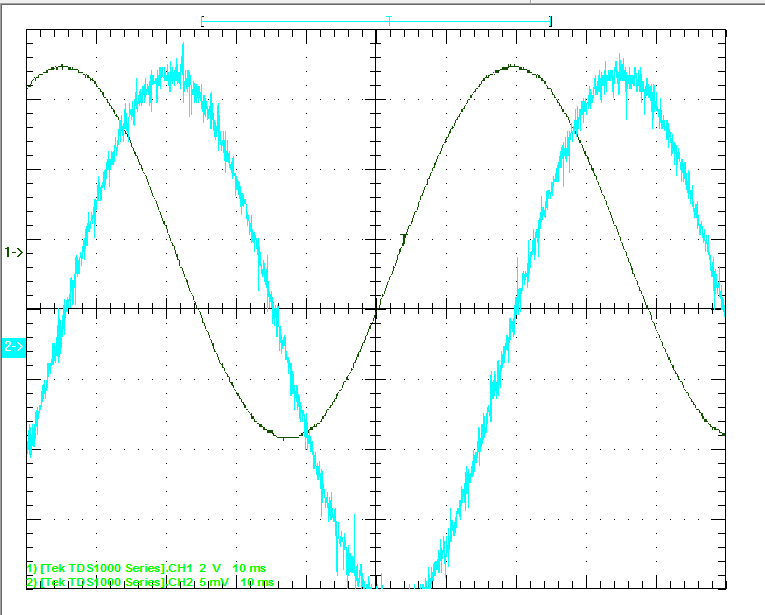
\includegraphics[width=\linewidth]{./Images/comparison.png}
  \label{fig:parallel_diagram}
  \caption{Comparison between waveforms of source voltage and capacitor voltage, scaled up to show phase difference.}
  \end{center}
  \par\end{centering}
  \end{figure}

  \begin{figure}[h!]
  \begin{centering}
  \begin{center}
  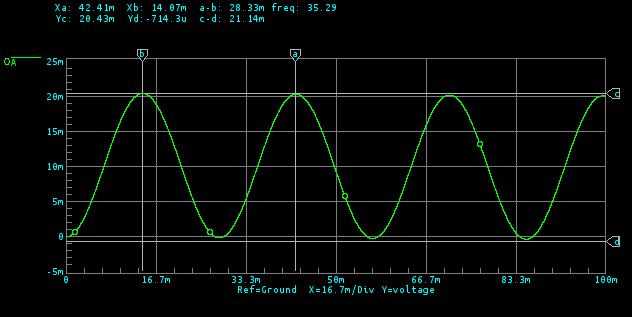
\includegraphics[width=\linewidth]{./Images/waveform.png}
  \label{fig:theory_wave}
  \caption{Theoretical capacitor voltage, as modeled in Circuit Maker 6.0}
  \end{center}
  \par\end{centering}
  \end{figure}

\section{Results}
\begin{table}[h!]
\centering{}
\caption{Measured vs. Theoretical Results from Capacitor Voltage Measurements}
\label{tb:meas_err}
\begin{tabular}{|c|c|c|c|}
\hline
\textbf{Parameter}	&\textbf{Measured Value}		&\textbf{Theoretical Value}	&\textbf{Percent Difference}	\\ \hline
$V$ Peak to Peak	&23.4 mV				&21.14mV 			&10\%				\\ \hline
Period			&28.44 ms				&28.33 mS  			&0.39\% 			\\ \hline
\end{tabular}
\end{table}

Although the resonant frequency for this circuit, given by $f_0 = 1/2\pi\sqrt{LC}$, was approximately 82.3 Hz, sweeping the circuit through a range of frequencies did not produce resonance or noticeable change the phase shift between the source and the capacitor voltages. Variation of other parameters, such as peak to peak voltage and wave type, likewise did not have an effect on the phase shift.

However, it was expected that the capacitor voltage would lag the source voltage by $90^{\circ}$, and the results were within 1.5\% of theory. The expression for the voltage across the capacitor, $(X_c/Z)V_{\text{max}}\sin(\omega t- \pi/2)$, shows that while the amplitude is frequency-dependent, the phase shift is not, which helps explain the aforementioned results.
%Comment on phase shift and voltage level.

\appendices{}

\section{Circuit Photograph}\label{append:deriv}

\begin{figure}[h!]
  \begin{centering}
  \begin{center}
  \includegraphics[width=\linewidth]{./Images/real_circuit.png}
  \label{fig:real_circuit}
  \caption{Photograph of Circuit Used}
  \end{center}
  \par\end{centering}
  \end{figure}

%\bibliographystyle{plain}
%\bibliography{physbib}

\end{document}